\documentclass[11pt]{article} 
\usepackage[french]{babel}
\usepackage[T1]{fontenc}
\usepackage[lmargin=1in,rmargin=1in,tmargin=1in,bmargin=1in]{geometry}
\usepackage{amsfonts,amsmath, amssymb,array}
\usepackage{graphicx}
\usepackage{titlesec}
\usepackage{filecontents} 
\usepackage{amsmath}


\titleclass{\subsubsubsection}{straight}[\subsection]

\newcounter{subsubsubsection}[subsubsection]
\renewcommand\thesubsubsubsection{\thesubsubsection.\arabic{subsubsubsection}}


\titleformat{\subsubsubsection}
  {\normalfont\normalsize\bfseries}{\thesubsubsubsection}{1em}{}
\titlespacing*{\subsubsubsection}
{0pt}{3.25ex plus 1ex minus .2ex}{1.5ex plus .2ex}

\titleformat{\paragraph}
  {\normalfont\normalsize\bfseries}{\theparagraph}{1em}{}
\titlespacing*{\paragraph}
{0pt}{3.25ex plus 1ex minus .2ex}{1.5ex plus .2ex}

\makeatletter
\renewcommand\subparagraph{\@startsection{subparagraph}{6}{\parindent}%
  {3.25ex \@plus1ex \@minus .2ex}%
  {-1em}%
  {\normalfont\normalsize\bfseries}}
\def\toclevel@subsubsubsection{4}
\def\toclevel@paragraph{5}
\def\toclevel@paragraph{6}
\def\l@subsubsubsection{\@dottedtocline{4}{7em}{4em}}
\def\l@paragraph{\@dottedtocline{5}{10em}{5em}}
\def\l@subparagraph{\@dottedtocline{6}{14em}{6em}}
\makeatother
\newcommand{\HRule}{\rule{\linewidth}{0.5mm}}

\setcounter{secnumdepth}{4}
\setcounter{tocdepth}{4}

%\input{mymathsym}
%% symboles mathématiques
\DeclareMathOperator*{\argmax}{arg\,max}


\newcommand{\E}{\mathbb{E}}
\newcommand{\Pro}{\mathbb{P}}
\newcommand{\Rset}{\mathbb{R}}
\newcommand{\Nset}{\mathbb{N}}	

\newcommand{\cB}{\mathcal{B}}
\newcommand{\cL}{\mathcal{L}}
\newcommand{\cN}{\mathcal{N}}



\newcommand{\bsX}{\boldsymbol{X}}
\newcommand{\bsx}{\boldsymbol{x}}
\newcommand{\bsy}{\boldsymbol{y}}
\newcommand{\bsp}{\boldsymbol{p}}
\newcommand{\bsz}{\boldsymbol{z}}
\newcommand{\bsk}{\boldsymbol{k}}
\newcommand{\bst}{\boldsymbol{t}}
\newcommand{\bsA}{\boldsymbol{A}}
\newcommand{\bsh}{\boldsymbol{h}}
\newcommand{\bsW}{\boldsymbol{W}}
\newcommand{\bsI}{\boldsymbol{I}}


\newcommand{\ciz}{\textit{z}}
\newcommand{\cif}{\textit{f}}
\newcommand{\ciy}{\textit{y}}
\newcommand{\cih}{\textit{h}}
\newcommand{\cil}{\textit{l}}
\newcommand{\cik}{\textit{k}}
\newcommand{\ciQ}{\textit{Q}}
\newcommand{\cia}{\textit{a}}
\newcommand{\cib}{\textit{b}}
\newcommand{\ciR}{\textit{R}}
\newcommand{\cir}{\textit{r}}
\newcommand{\cit}{\textit{t}}
\newcommand{\cim}{\textit{m}}



\newcommand{\sumn}{\sum_{i=1}^{n}}
\newcommand{\sumK}{\sum_{k=1}^{K}}
\newcommand{\sumR}{\sum_{r=1}^{R}}
\newcommand{\sumttn}{\sum_{t=2}^{n}}
\newcommand{\sumtn}{\sum_{t=1}^{n}}
\newcommand{\sumlK}{\sum_{l=1}^{K}}


\newcommand{\bX}{\mathbf{X}}
\newcommand{\bY}{\mathbf{Y}}
\newcommand{\bZ}{\mathbf{Z}}
\newcommand{\bK}{\mathbf{K}}
\newcommand{\bA}{\mathbf{A}}
\newcommand{\bR}{\mathbf{R}}



\newcommand{\bstheta}{\boldsymbol{\theta}}
\newcommand{\bsPsi}{\boldsymbol{\Psi}}
\newcommand{\bsbeta}{\boldsymbol{\beta}}
\newcommand{\betakT}{\boldsymbol{\beta}_{k}^{T}}
\newcommand{\betaT}{\boldsymbol{\beta}^{T}}



\begin{document}
\begin{titlepage}
\begin{center}
	\begin{figure}
		\begin{minipage}[c]{.46\linewidth}
      			\begin{flushleft}		
			
\includegraphics[height=3cm]{unicaen.png}
	  		\end{flushleft}
    		\end{minipage}
		
    \end{figure}
    \textsc{\LARGE Université de Caen Normandie}\\[5cm]
    
    % Title
    \HRule \\[0.4cm]
    { \huge \bfseries Régression à l'aide du modèle de Markov caché à effets mixtes }

    \HRule \\[7.5cm]


    % Author and supervisor
    
    \begin{minipage}{0.4\textwidth}
      \begin{flushleft} \large
        \emph{Auteurs :}S.Blin A.Bourjal C.Champarou\\
        \emph{M2 Statistiques Appliquées et Analyse Décisionnelle}
      \end{flushleft}
    \end{minipage}
    \begin{minipage}{0.4\textwidth}
      \begin{flushright} \large
        \emph{Tuteur projet :} M. \textsc{F.Chamroukhi}\\
      \end{flushright}
    \end{minipage}

    \vfill

    % Bottom of the page
    Année universitaire 2018-2019


\end{center}
\end{titlepage}

\newpage
\section*{Introduction}

Les modèles de Markov cachés (HMM) constituent une classe de modèles de données latentes appropriés aux données séquentielles. Ils sont largement utilisés dans de nombreux domaines d’application, notamment la reconnaissance vocale, l’analyse d’images, la prédiction de séries temporelles .\\


\begin{figure}[h]
\begin{center}
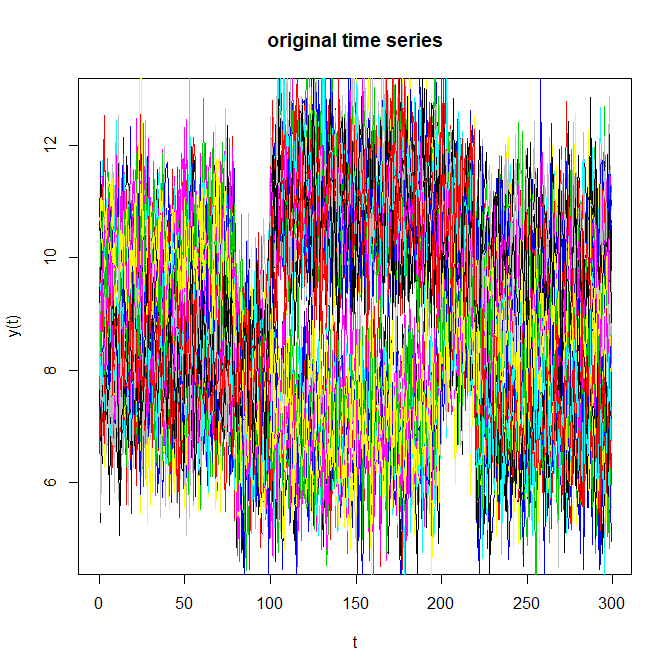
\includegraphics[height=8cm]{data1.png}
\end{center}
\end{figure}

\newpage
\tableofcontents
\newpage
\section*{Modèle}

Dans un HMM, l’observation la séquence (ou une série chronologique) $\bsy_{i} = (\bsy_{i1},\ldots, \bsy_{im})$ est supposée être régie par une séquence d'états cachés$\bsz_{i} = (\bsz_{i1},\ldots, \bsz_{im})$ où la variable aléatoire discrète$\bsz_{ij}=\{1, \dots , R\}$ représente l'état non observé associé à  $\bsy_{ij}$ à l'instant $\bst_{1}$. La séquence d'état $\bsz$ est généralement supposée être une chaîne de Markov homogène du premier ordre, c'est-à-dire que l'état actuel, car la séquence d'états précédente ne dépend que de l'état précédent. Formellement nous avons:

\begin{equation}
\bsp(\bsz_{ij} | \bsz_{i,j-1},  \bsz_{i,j-2}, \dots, \bsz_{i1}) = \bsp(\bsz_{ij} | \bsz_{i,j-1}) \forall j > 1
\end{equation}

Le modèle proposé suppose que chaque série chronologique yi est issu d’un des $\bK$ clusters où, au sein de chaque cluster $\bsk (\bsk = 1,\dots, \bK)$, chaque série temporelle est générée par $\bR$ régimes polynomiaux non observés. La transition d'un régime à un autre est régi par un Markov homogène Chaîne de premier ordre. Formellement, la distribution d'une fois la série yi est définie par le mélange conditionnel suivant densité: 

\begin{equation}
\cif (\bsy_{i} | \bst ; \bsPsi) = \sumK \alpha_{k} \cif_{k} (\bsy_{i} | \bst ; \bsPsi_{k}),
\end{equation}

où chaque composante de densité $\cif_{k}(.)$ associée à la $\bsk_{th}$ cluster est un modèle de régression polynomial HMM. Dans ce contexte de clustering avec régression HMM, en fonction du cluster $\bsh_{i} = \bsk$, la série chronologique  $\bsy_{i} = (\bsy_{i1},\ldots, \bsy_{im})$ est supposée être généré par le modèle de régression suivant:  

\begin{equation}
\bsy_{ij}=\beta_{kx_{ij}}^{T} \bst_{j} + \sigma_{kx_{ij}}\epsilon_{ij} \qquad (j = 1,\ldots, \cim)
\end{equation}

\section{Paramètre}

$\beta_{kr}$ est le vecteur des coefficients dimensionnels $(\bsp + 1)$ du r ième modèle de régression polynomiale du groupe $\bsk$\\

$\sigma_{kr}^{2}$ est sa variance de bruit associée et les $\sigma_{ij}$ sont des variables aléatoires indépendantes réparties selon une distribution gaussienne à moyenne nulle et à variance unitaire. La séquence d'état cachée $\bsz_{i} = (\bsz_{i1},\ldots, \bsz_{im})$ est supposée être une chaîne de Markov de paramètres $(\bsp_{k}, \bsA_{k})$.\\

Le modèle proposé est illustré par la représentation graphique de la figure 1. Chaque composant la densité est donc paramétrée par le vecteur paramètre  
\begin{equation}
\phi_{k} = (\bsp_{k},\bsA_{k}, \beta_{k1},\dots, \beta_{kR}, \sigma_{k1}^{2},\dots, \sigma_{kR}^{2})
\end{equation}

\section{Estimation} 

\subsection{Estimation par Maximum de vraisemblance}

L’estimation des paramètres est réalisée en maximisant la log des données observées - probabilité de $\bsPsi$: \\

\begin{equation}
\begin{aligned}
\cL (\bsPsi) &= \text{log}\ \bsp(\bsy_{1},\dots,\bsy_{n} |\bst;\bsPsi )\\
 &= \text{log} \ \prod_{i=1}^{n}\bsp(\bsy_{i}|\bst;\bsPsi) \\
&= \sumn \text{log} \ \sumK \alpha_{k} \sum_{x_{i}}\bsp(\ciz_{i1}\pi_{k}) \prod_{j=2}^{m}\bsp(\bsz_{ij}|\bsz_{i,j-1};\bsA_{k}) \prod_{j=1}^{m}\cN ( \bsy_{ij} ;\beta_{kx_{ij}}^{T}\bst_{j}, \sigma_{kx_{ij}}^{2})
\end{aligned}
\end{equation}

La maximisation de ce log-vraisemblance ne peut pas être effectuée sous une forme fermée. Nous le maximisons de manière itérative en utilisant un algorithme EM dédié. Avec cette spécification de l'algorithme EM, les données complètes pour le modèle proposé sont constituées de l'ensemble de courbes observées $\bY = (\bsy_{1},\dots, \bsy_{n})$, de leurs étiquettes de grappes correspondantes $\bsh = (\cih_{1},\dots, \cih_{n})$. et la matrice des étiquettes de régime (état) $\bsh = (\bsz_{1},\dots, \bsz_{n})$, $\bsz_{i}$ étant le séquence d'état cachée associée à $\bsy_{i}$. Les données complètes La probabilité de $\Psi$ est donc donnée par: \\

\begin{equation}
\begin{aligned}
\bsp(\bY,\bsh,\bZ|\bst;\bsPsi) &= \bsp(\bsh) \ \bsp(\bY,\bZ|\bsh,\bst;\bsPsi) \\
 &=  \bsp(\bsh) \ \bsp(\bZ|\bsh,\bst;\bsPsi) \ \bsp(\bY|\bsh,\bZ,\bst;\bsPsi)
\end{aligned}
\end{equation}



\subsection{Estimation  par l'ALgorithme EM}

Dans cette etape on Calcule la log-vraisemblance complète attendue pour les données complètes:

\begin{equation}
\begin{aligned}
\cL_{c}(\bsPsi) = \text{log} \ \bsp(\bY,\bsh,\bZ|\bst;\bsPsi &= \sumK \Bigg[ \sumn \cih_{ik} \ \text{log} \ \alpha_{k} + \sumn \sumR\cih_{ik}\bsz_{i1kr} \ \text{log} \ \pi_{kr} \\ 
&+ \sumn \sum_{j=2}^{m} \sum_{l=1}^{R} \cih_{ik}\bsz_{ijkr}\bsz_{i(j-1)kr} \ \text{log} \ \bA_{klr} \\
&+ \sumn \sum_{j=1}^{m} \sumR \cih_{ik}\bsz_{ijkr}\cN ( \bsy_{ij} ;\beta_{kr}^{T}\bst_{j}, \sigma_{kr}^{2}) \Bigg]
\end{aligned}
\end{equation}


\subsubsection{Etape E}

Calculer la loglikistence attendue pour les données complètes en fonction de la série temporelle $\bY$, du vecteur temporel $\bst$ et de la valeur actuelle du paramètre $\bsPsi$ , notée $\bsPsi^{(q)}$: 

\begin{equation}
\ciQ ( \bsPsi , \bsPsi^{(q)}) = \E [ \cL_{c} (\bsPsi) | \bY,\bst ; \bsPsi^{(q)} ]
\end{equation}

Ce qui nous donne ensuite : \\

\begin{equation}
\ciQ ( \bsPsi , \bsPsi^{(q)}) = \ciQ_{1}(\alpha_{k}) + \sumK [ \ciQ_{2}(\pi_{k}, \bA_{k}) + \ciQ_{3}(\beta_{kr}, \sigma_{kr}^{2})],
\end {equation}

où \\

\begin{equation}
\begin{array}{c}
\ciQ_{1}(\alpha_{k}) = \sumK \sumn \tau_{ik}^{(q)} \ \text{log} \ \alpha_{k}, \\
\\
\ciQ_{2}(\pi_{k},\bA_{k}) = \sumR \sumn \tau_{ik}^{(q)} [ \gamma_{ijkr}^{(q)} \ \text{log} \ \pi_{kr} + \sum_{j=2}^{m} \sum_{l=1}^{R} \epsilon_{ijkr}^{(q)} \ \text{log} \ \bA_{klr}],\\
\\
\ciQ_{3}(\beta_{kr},\sigma_{kr}^{2})= \sumR \sumn \sum_{j}^{m} \tau_{ik}^{(q)}  \gamma_{ijkr}^{(q)} \  \text{log} \ \cN (\bsy{ij} ; \beta_{kr}^{T} \bst_{j}
\end{array}
\end{equation}

où \\

\begin{itemize}
\item
$ \tau_{ik}^{(q)} = \bsp(\bsh_{i} = \bsk| \bsy_{i},\bst ; \bsPsi^{q})$ qui est la probabilité à postériori de la classe $\cik$; \\

\item
$\gamma_{ijkr}^{(q)} = \bsp(\ciz_{ijk} = \cir| \bsy_{i},\bst ; \bsPsi_{k}^{q})$ qui est la probabilité à postériori du $\cik$th régime polynomiale pour la $\cik$th classe, \\

\item
$\epsilon_{ijkrl}^{(q)}  = \bsp(\ciz_{ijk} = \cir, \ciz_{i(j-1)k} = \cil | \bsp_{i}, \bst ; \bsPsi_{k}^{(q)})$ qui est la probabilité jointe d'avoir le régime $\cir$ à un temps $\bst_{j}$  et le regime $\cil$ à un temps $\bst_{j-1}$ dans la classe $\bsk$

\end{itemize}

Ainsi, dans l'équation ci-dessus, il nous faut calculer les probabilités à postériori de $\epsilon_{ijklr}^{(q)}$,  $\gamma_{ijkr}^{(q)}$ et $\tau_{ik}^{(q)}$. Ces dernier calculer par les récursions du forward-backward. \\



\paragraph{Forward-Backward}

Le processus du forward calcul recursivement les probabilités :\\

\begin{equation}
\cia_{ijkr} =\bsp ( \bsy_{i1},\ldots,\bsy_{ij}, \ciz_{ijk} = \cir | \bst ; \bsPsi_{k})
\end{equation}

Dans un autre temps, le processus du backward calcul les probabilités à partir des temps $(\bst+1, \ldots, n)$\\

\begin{equation}
\cib_{ijkr} =\bsp ( \bsy_{i,j+1},\ldots,\bsy_{im} | \ciz_{ijk} = \cir| \bst ; \bsPsi_{k})
\end{equation}

Ce qui nous permet de calculer les probabilités de $\gamma_{ijkr}^{(q)}$ et $\epsilon_{ijklr}^{(q)}$.\\

\begin{equation}
\gamma_{ijkr}^{(q)} = \frac{ \cia_{ijkr}^{(q)} \cib_{ijkr}^{(q)}}{ \sum_{l=1}^{R} \cia_{ijkl}^{(q)} \cib_{ijkl}^{(q)}}
\end{equation}

et \\

\begin{equation}
\epsilon_{ijklr}^{(q)} = \frac{\cia_{i(j-1)l}^{(q)} \bsA_{klr}^{(q)} \cN (\bsy_{ij} ; \beta_{kr}^{(q)T} \bst_{j}, \sigma_{kr}^{(q)2}) \cib_{ijkr}^{(q)}}{\sum_{r,l=1}^{R} \cia_{i(j-1)lk}^{(q)} \bA_{klr}^{(q)} \cN (\bsy_{ij} ; \beta_{kr}^{(q)T} \bst_{j}, \sigma_{kr}^{(q)2}) \cib_{ijkr}^{(q)}}
\end{equation}


La probabilité à postériori de la classe $\tau_{ik}^{(q)}$ que la série temporelle $\bsy_{i}$ appartient à la classe $\bsk$ est donné quant à elle par : \\

\begin{equation}
\tau_{ik}^{(q)}= \frac{\alpha_{k}^{(q)} \cif_{k}(\bsy_{i} | \bst ; \bsPsi_{k}^{(q)})}{\sum_{k'=1}^{K} \alpha_{k'}^{(q)} \cif_{k}(\bsy_{i} | \bst ; \bsPsi_{k'}^{(q)}) }
\end{equation}


\subsubsection{Etape M}

Dans cette étape, la valeur du paramètre est mis à jour en maximisant la valeur loglikistence des données complètes attendue par rapport à, à savoir: 

\begin{equation}
\bsPsi^{(q+1)}  = \underset{\bsPsi}{\argmax}  \ \ciQ ( \bsPsi, \bsPsi^{(q)} ) 
\end{equation}

La maximisation de $\ciQ$ peut être réalisé en maximisant les fonctions $\ciQ_{1}$,  $\ciQ_{2}$ et  $\ciQ_{3}$. La maximisation de  $\ciQ_{1}$ avec $\alpha_{k}$ est l'un des modèles mixte les plus standard. Les mises à jours étant donné par : \\

\begin{equation}
\alpha_{k}^{(q+1)} = \frac{\sumn \tau_{ik}^{(q)}}{n}
\end{equation}

La maximisation de $\ciQ_{2}$ se fait grâce aux paramètres $(\pi_{k}, \bA)$ qui correspond à un version pondéré de la mise à jour des paramètres dans la chaîne de Markov dans le modèle standart de HMM. Ces paramètres deviennent ainsi :\\


\begin{equation}
\pi_{kr}^{(q+1)} = \frac { \sumn \tau_{ik}^{(q)} \gamma_{i1kr}^{(q)}}{ \sumn \tau_{ik}^{(q)}}
\end{equation}

et \\

\begin{equation}
\bA_{klr}^{(q+1)}= \frac { \sumn \sum_{j=2}^{m} \tau_{ik}^{(q)} \epsilon_{ijklr}^{(q)}}{\sumn \sum_{j=2}^{m} \tau_{ik}^{(q)} \gamma_{ijkr}^{(q)}}
\end{equation}

La maximisation de $\ciQ_{3}$ se fait grâce aux paramètres de la regression $\beta_{kr}$ pour $\bsk = 1,\ldots,\bK$ et $\cir = 1,\ldots,\ciR$. Le paramètre mis à jour est donné par : \\

\begin{equation}
\beta_{kr}^{(q+1)} = \Big[ \bsX^{T}(\sumn \tau_{ik}^{(q)} \bsW_{ikr}^{(q)}) \bsX \Big]^{-1}  \bsX^{T}(\sumn \tau_{ik}^{(q)} \bsW_{ikr}^{(q)} \bsy_{i})
\end{equation}

où $\bsW_{ikr}^{(q)}$ est une matrice diagonale $\cim \times \cim$ avec pour éléments diagonals les poids $\{ \gamma_{ijkr}^{(q)}; j= 1,\ldots,\cim \}$ \\

Ansi, la maximisation de $\ciQ_{3}$ en respectant le bruit des variances $\sigma_{kr}^{2(q+1)}$ consiste à la formule : \\

\begin{equation}
\sigma_{kr}^{2(q+1)}= \frac{\sumn \tau_{ik}^{(q)} || \sqrt{\bsW_{ikr}^{(q)}} (\bsy_{i} - \bsX \beta_{kr}^{(q+1)})||^{2}}{\sumn \tau_{ik}^{(q)} \ \text{trace} \ ( \bsW_{ikr}^{(q)})}
\end{equation}


\newpage
\section{Application}

Dans cette section, nous présenterons l'utilisation de la régression à l'aide du modèle de Markov à effets mixtes sur des données simulées. Celle-ci sont représenté sur le graphe suivant : \\

\begin{figure}[h]
\begin{center}
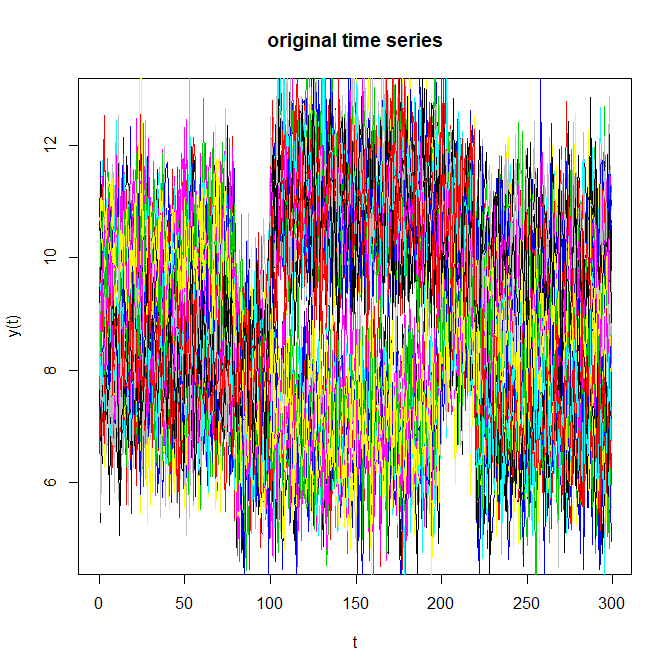
\includegraphics[height=8cm]{data1.png}
\end{center}
\end{figure}

Nous supposons avec ce graphique que les données peuvent être séparées en 3 séries temporelles disctinctes (voir graphique ci-dessous).\\

\begin{figure}[h]
\begin{center}
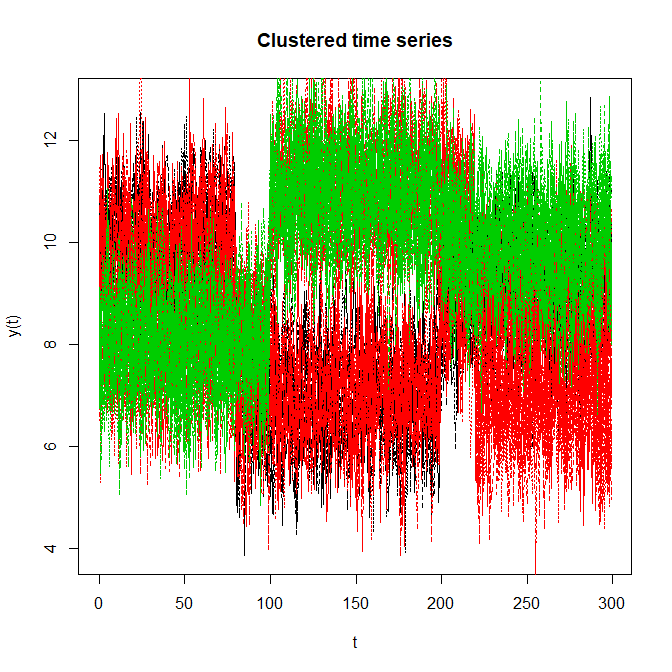
\includegraphics[height=8cm]{clustering.png}
\end{center}
\end{figure}

Ensuite, nous séparons les 3 séries temporelles que nous ajusterons séparement grâce à un modèle de Markov caché.

\begin{figure}[h]
\begin{center}
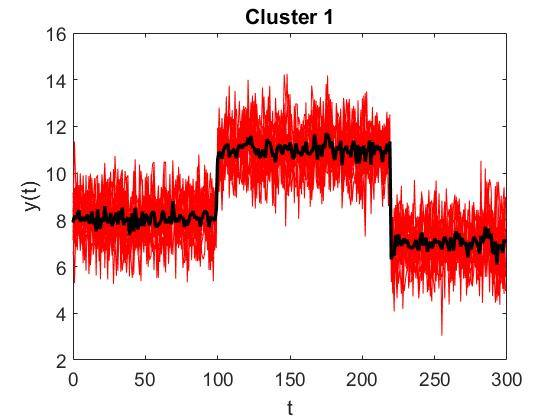
\includegraphics[height=8cm]{cl1.jpg}
\end{center}
\end{figure}

Le graphique ci-dessus montre une première série temporelle avec un ajustement avec une régression à l'aide du modèle de Markov caché.\\

\begin{figure}[h]
\begin{center}
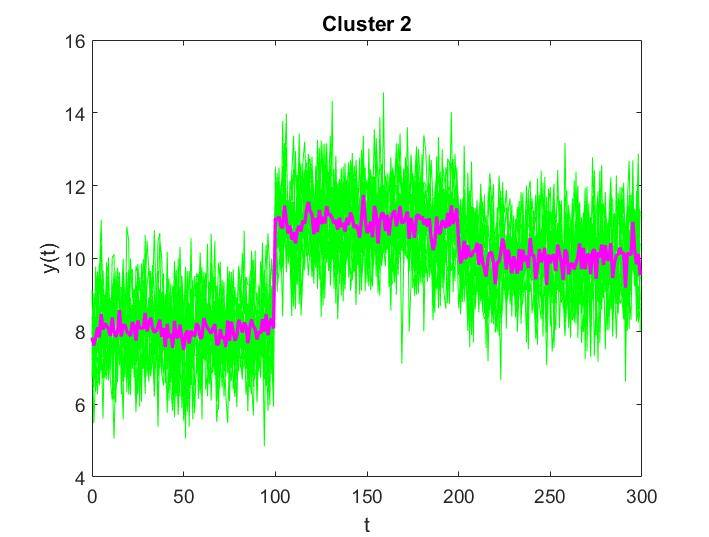
\includegraphics[height=8cm]{cl2.jpg}
\end{center}
\end{figure}

Le graphique ci-dessus montre une seconde série temporelle avec un ajustement avec une régression à l'aide du modèle de Markov caché.\\

\newpage
\begin{figure}[h]
\begin{center}
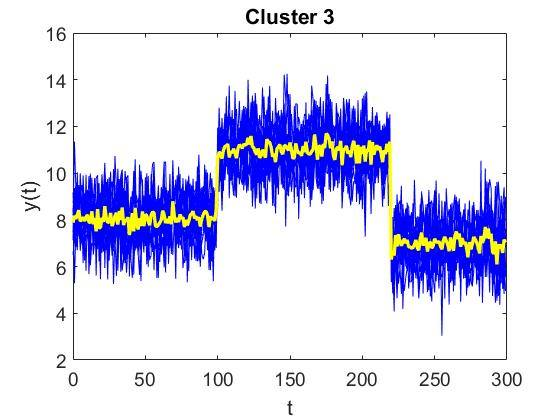
\includegraphics[height=8cm]{cl3.jpg}
\end{center}
\end{figure}

Le graphique ci-dessus montre une troisème série temporelle avec un ajustement avec une régression à l'aide du modèle de Markov caché.\\


\end{document}